\chapter{分离混合物}\label{ch:g3:separating-mixtures}

暴风雨过后，路上的积水呈棕色，里面混着
泥土、沙子和碎树叶。而从厨房水龙头流出的水
却是清澈的，它也曾是雨水，流进河里之前。怎样
才能让浑水重新变干净？混在一起的东西可以
被分开。本章逐一介绍各种分离方法。

\begin{recall}
混合就是把不同的东西放在一起。糖或盐这类固体
溶于水中：它从视线中消失，清澈的液体
就是溶液。溶解的固体仍然存在：水干了以后，
固体会留下来。沙子和泥土不能溶解
（见\cref{ch:g2:mixing-and-dissolving}）。
\end{recall}

\section{用手分拣和筛分}

当混合物中的颗粒大到能看见、能拿起时，
最简单的分离方法是用手挑：葡萄干可以从
什锦麦片中一颗一颗地挑出来。颗粒太多时，就由筛子
帮我们分拣。

\begin{definition}[筛分]\label{def:g3:separating-mixtures:sieve}
\emph{筛分}\index{筛分}是用筛子把混合物中的颗粒
按大小分开：筛子是一张布满孔洞的网或板。小颗粒
从孔中漏下，大颗粒则留在筛子里。
\end{definition}

\begin{example}[碎石和沙子]\label{ex:g3:separating-mixtures:gravel}
一位建筑工人把碎石和沙子的混合物放在筛子上抖动。细沙
漏到下面堆成一堆；碎石则留在筛网上。
\end{example}

\begin{omfigure}
\begin{tikzpicture}[font=\small]
  % the sieve: a mesh bowl
  \fill[pattern=crosshatch, pattern color=black!45] (-1.6,2.6) arc[start angle=180,
    end angle=360, x radius=1.6, y radius=0.7] -- cycle;
  \draw[black!70, line width=0.8pt] (-1.6,2.6) arc[start angle=180, end angle=360,
    x radius=1.6, y radius=0.7];
  \draw[black!70, line width=0.8pt] (-1.75,2.6) -- (1.75,2.6);
  \draw[black!70, line width=1.4pt] (1.75,2.6) -- (3.0,2.85);
  % gravel kept in the sieve
  \foreach \x/\y/\r in {-0.9/2.25/0.17,-0.45/2.12/0.2,0.05/2.08/0.18,0.5/2.13/0.21,
                        0.95/2.28/0.16,-0.2/2.42/0.15,0.3/2.43/0.17}
    \fill[black!45, draw=black!65] (\x,\y) circle (\r);
  % sand falling
  \foreach \x/\y in {-0.4/1.6,0.1/1.4,0.4/1.7,-0.15/1.15,0.25/1.0,-0.5/0.95,0.0/0.75}
    \fill[orange!60!brown] (\x,\y) circle (0.05);
  % the heap of sand in a bowl
  \fill[orange!45!brown!70] (-1.0,0.12) .. controls (-0.5,0.55) and (0.5,0.55)
    .. (1.0,0.12) -- cycle;
  \draw[black!70, line width=0.8pt] (-1.5,0.5) .. controls (-1.3,0) and (1.3,0)
    .. (1.5,0.5);
  \node[anchor=west] at (2.0,2.2) {碎石留在筛子里};
  \node[anchor=west] at (2.0,1.25) {沙子从孔中漏下};
  \node[anchor=west] at (2.0,0.3) {一堆沙子};
\end{tikzpicture}

{\small 用筛子分离碎石和沙子的混合物：颗粒按
大小分开。}
\end{omfigure}

\begin{omfigure}
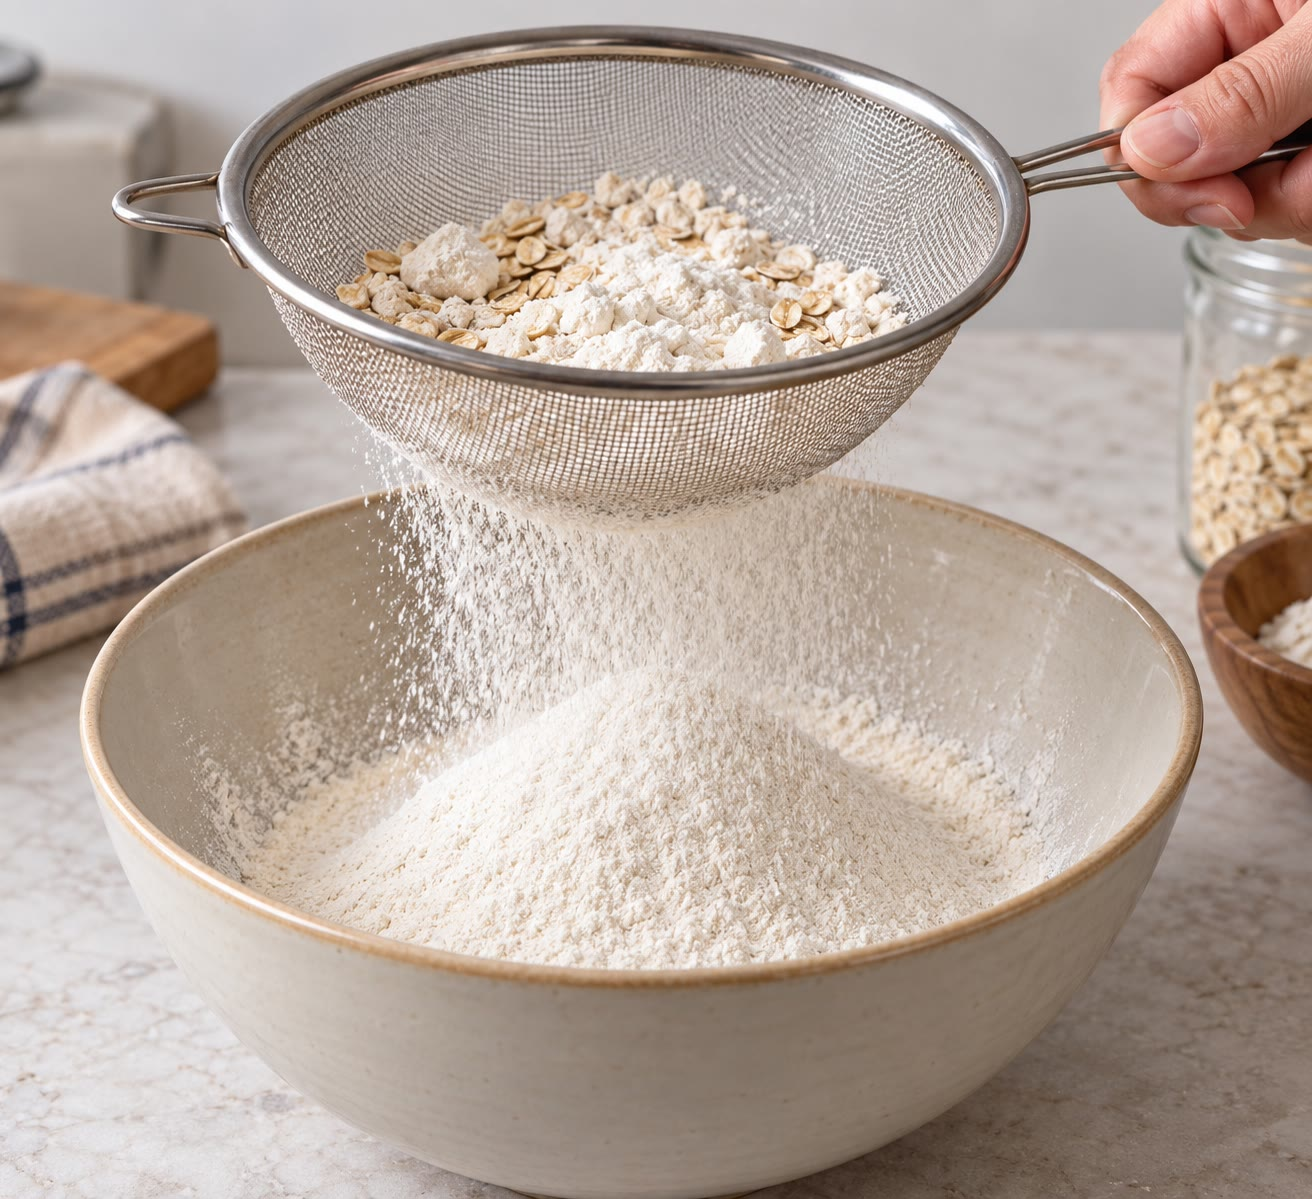
\includegraphics[width=0.55\linewidth]{images/book1/ai/g3-kitchen-sieve.jpg}

{\small 厨房里的筛子：细面粉漏过去，
结块的留在筛子里。}
\end{omfigure}

\section{沉降与倾析}

\begin{definition}[沉降与倾析]\label{def:g3:separating-mixtures:decant}
水与不溶于水的固体的混合物可以静置
一段时间：固体会慢慢下沉到底部。这种现象称为
\emph{沉降}\index{沉降}。待其沉降后，上层的清水
可以小心地倒入另一个容器中，把固体留在
原处：这种操作称为\emph{倾析}\index{倾析}。
\end{definition}

\begin{omfigure}
\begin{tikzpicture}[font=\small]
  % 1: stirred, cloudy
  \pic at (0,0) {beaker={0.7}{brown!28}};
  \foreach \x/\y in {-0.5/0.3,-0.2/0.6,0.3/0.4,0.5/0.9,-0.4/1.0,0.1/1.2,0.4/0.15,
                     -0.1/0.25,0.2/0.8,-0.55/0.7}
    \fill[brown!60] (\x,\y) circle (0.03);
  \node[anchor=north, align=center] at (0,-0.15) {搅拌后：\\ 浑浊};
  \draw[->, thick, omProp] (1.1,1.0) -- (2.4,1.0);
  % 2: settled
  \pic at (3.5,0) {beaker={0.7}{omWater!80}};
  \fill[brown!60] (2.7,0) rectangle (4.3,0.25);
  \draw[omGlass, line width=0.7pt] (2.7,0.25) -- (2.7,0) -- (4.3,0) -- (4.3,0.25);
  \node[anchor=north, align=center] at (3.5,-0.15) {静置：\\ 泥土已沉降};
  \draw[->, thick, omProp] (4.6,1.0) -- (5.9,1.0);
  % 3: decanted
  \pic at (7.0,0) {beaker={0.1}{omWater!80}};
  \fill[brown!60] (6.2,0) rectangle (7.8,0.25);
  \draw[omGlass, line width=0.7pt] (6.2,0.25) -- (6.2,0) -- (7.8,0) -- (7.8,0.25);
  \pic at (9.2,0) {beaker={0.58}{omWater!80}};
  \node[anchor=north, align=center] at (8.1,-0.15) {倾出：清水 \\ 在右边，泥土留在原处};
\end{tikzpicture}

{\small 沉降，然后倾析泥土与水的混合物。}
\end{omfigure}

\begin{remark}[沉降需要时间]\label{rem:g3:separating-mixtures:time}
较大、较重的颗粒几分钟内即可沉降；极细的黏土
可能需要一天或更长时间，其间水仍会略显浑浊。倾析
并不能去除全部颗粒：少量浑浊物会随清水一起倒出。
\end{remark}

\section{过滤}

\begin{definition}[过滤与滤液]\label{def:g3:separating-mixtures:filter}
\emph{过滤}\index{过滤}是指把混合物倒过滤器：
 滤纸、布或一层沙子，其上的孔眼很小，
 固体颗粒无法穿过。固体留在滤器上，
 穿过的清澈液体称为
 \emph{滤液}\index{滤液}。
\end{definition}

\begin{omfigure}
\begin{tikzpicture}[font=\small, scale=1.4]
  \pic[transform shape] at (0,0) {beaker={0.35}{omWater!80}};
  \pic[transform shape] at (0,1.4) {funnel={brown!55}};
  % muddy water waiting in the paper cone, above the soil
  \fill[brown!25] (-0.411,2.45) -- (0.411,2.45) -- (0.722,2.8) -- (-0.722,2.8) -- cycle;
  % drops of filtrate
  \foreach \y in {1.15,0.95} \fill[omDef!50] (0,\y) circle (0.04);
  \draw[<-, omProp, thick] (0.75,2.6) -- (2.0,2.9) node[right, text=black]
    {漏斗中的滤纸};
  \draw[<-, omProp, thick] (0.25,2.15) -- (2.0,2.2) node[right, text=black]
    {泥土留在滤纸上};
  \draw[<-, omProp, thick] (0.85,0.4) -- (2.0,0.6) node[right, text=black]
    {滤液：清水};
\end{tikzpicture}

{\small 用纸质滤器过滤浑浊的水。}
\end{omfigure}

\begin{inthelab}[过滤浑浊的水]
老师把一张圆形滤纸折成锥形，放在烧杯上方的
玻璃漏斗中。浑浊的水每次只倒入一点，
且绝不超过滤纸的边缘。清水滴入烧杯，
泥土在滤纸上形成一层褐色的土层。当
滤液浑浊时，说明滤纸破了，或水从边缘溢了出去。
\end{inthelab}

\begin{proposition}[过滤不能阻挡已溶解的物质]\label{prop:g3:separating-mixtures:dissolved}
滤纸能拦住未溶解的固体颗粒，
却拦不住已溶解的物质：盐水倒过滤纸后，
仍然一样咸，糖茶也仍然一样甜。
\end{proposition}

\begin{omfigure}
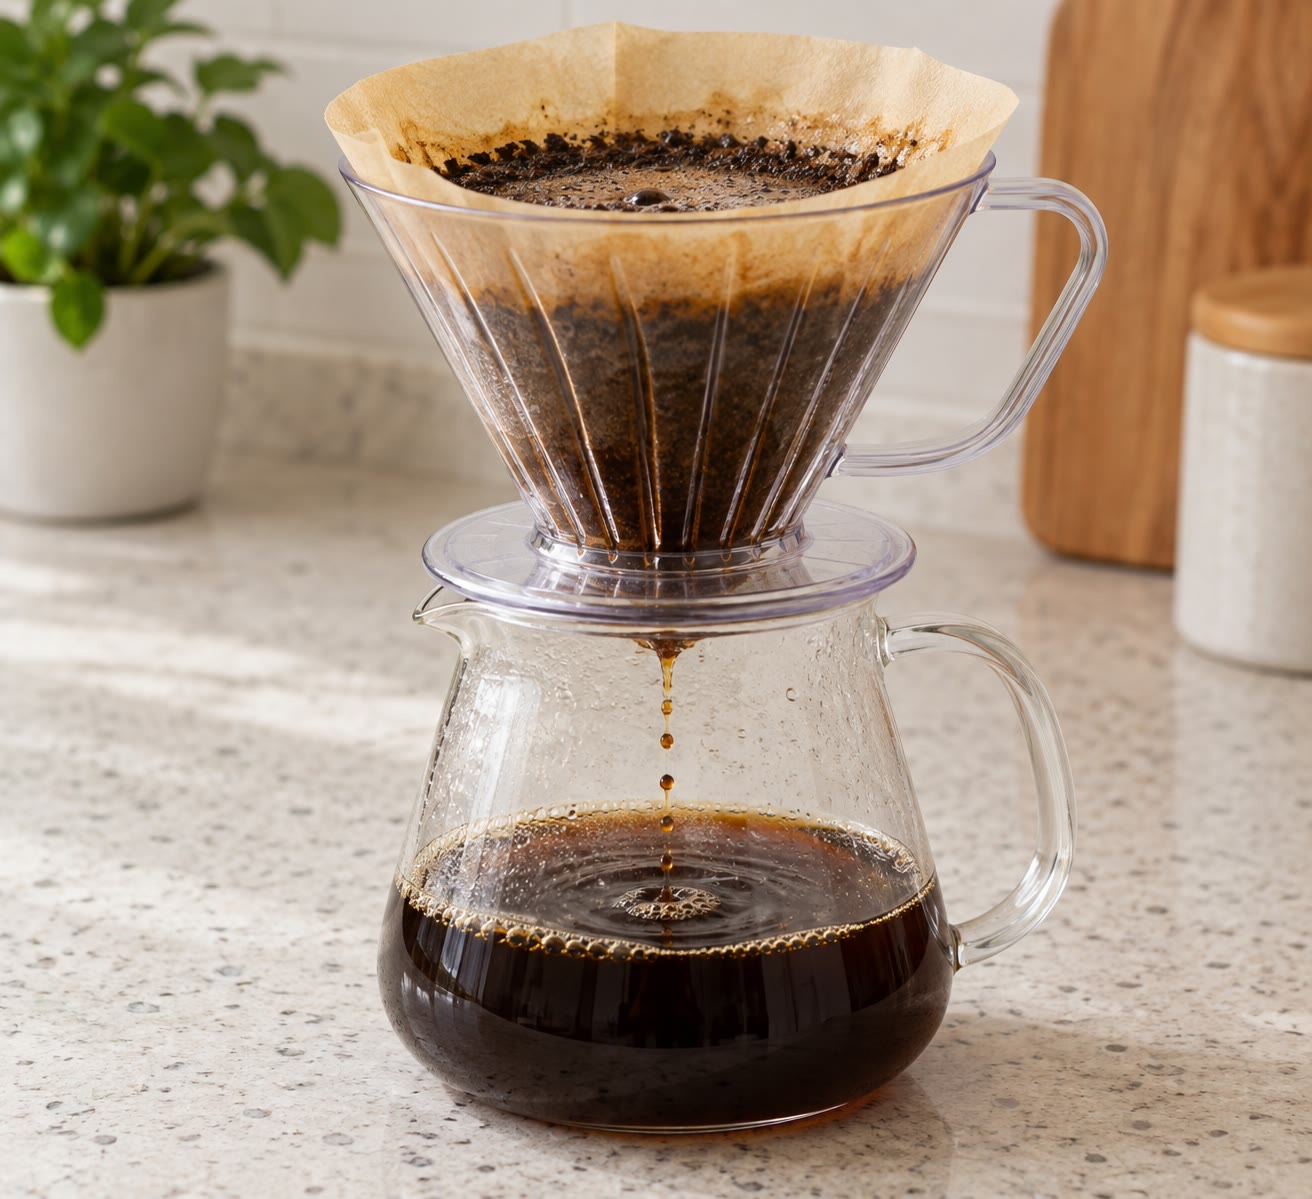
\includegraphics[width=0.5\linewidth]{images/book1/ai/g3-coffee-filter.jpg}

{\small 煮咖啡就是过滤：咖啡渣留在滤纸里，
咖啡是滤液。}
\end{omfigure}

\section{让水蒸发掉}

\begin{definition}[蒸发]\label{def:g3:separating-mixtures:evaporate}
要得到溶于水中的固体，可以让水自然干掉，
例如放在阳光下，或用文火加热，这种做法称为
\emph{蒸发}\index{蒸发}。水进入空气中，
固体则留在蒸发皿中。
\end{definition}

\begin{example}[从盐水中得到食盐]\label{ex:g3:separating-mixtures:salt}
将少量盐水倒入一个浅碟中，放在阳光充足的
窗台上。几天后水已经没有了，只剩下一层白色的
食盐结晶，即原先溶解在水中的食盐。
\end{example}

\begin{omfigure}
\begin{tikzpicture}[font=\small, scale=1.4]
  \pic[transform shape] at (0,0) {hotplate};
  \pic[transform shape] at (0,0) {evapdish={omWater!80}};
  \node[anchor=north, align=center] at (0,-0.6) {盐水，\\ 慢慢加热};
  \draw[->, thick, omProp] (1.5,0.3) -- (3.0,0.3) node[midway, above, text=black]
    {之后};
  \pic[transform shape] at (4.5,0) {hotplate};
  \pic[transform shape] at (4.5,0) {evapdish={white!85!black}};
  \foreach \x in {-0.45,-0.25,-0.05,0.15,0.35}
    \fill[white, draw=black!45, line width=0.2pt] (4.5+\x,0.12) rectangle ++(0.09,0.06);
  \node[anchor=north, align=center] at (4.5,-0.6) {水已蒸干，\\ 出现食盐晶体};
  \foreach \x in {-0.3,0,0.3} \draw[->, black!45, decorate,
    decoration={snake, amplitude=0.6pt, segment length=4pt}] (\x,0.7) -- (\x,1.4);
  \node[anchor=south] at (0,1.4) {水进入空气中};
\end{tikzpicture}

{\small 实验室中的蒸发：老师用电热板轻轻加热
蒸发皿，食盐留在皿中。}
\end{omfigure}

\section{哪种方法适用于哪种混合物？}

\begin{method}[选择分离方法]\label{met:g3:separating-mixtures:choose}
要分离一种混合物，可以问：
\begin{enumerate}
  \item 颗粒是否较大且大小不一？可用手拣，或
        筛分。
  \item 液体中是否有不溶的固体？让它
        沉降后倾析，或过滤得到较清的水。
  \item 液体中是否溶有固体？蒸发液体，
        固体留下。
\end{enumerate}
通常需要依次进行几个步骤。
\end{method}

\begin{example}[沙、盐与水]\label{ex:g3:separating-mixtures:three}
一个罐子里装着混有沙子和食盐的水。食盐已经溶解，
沙子则没有。
\begin{enumerate}
  \item 过滤：沙子留在滤纸上。
  \item 滤液清澈，但它是盐水。蒸发它，
        食盐留在蒸发皿中。
\end{enumerate}
依次使用两种方法，即可分别得到沙子和食盐。
\end{example}

\begin{example}[从河水中得到干净的水]\label{ex:g3:separating-mixtures:plant}
一座净水厂分几个步骤，使河水可以饮用：
\begin{enumerate}
  \item 河水流经滤网，滤网是一些大格栅，能挡住
        树枝、树叶和塑料，这是一种筛分；
  \item 河水流入大水池静置，泥沙沉到池底；
  \item 然后穿过厚厚的沙层过滤，沙层能拦住
        最细小的颗粒；
  \item 再加入少量能杀灭细菌的物质，
        使水在管道中保持安全。
\end{enumerate}
\end{example}

\begin{omfigure}
\begin{tikzpicture}[font=\small, node distance=0.45cm,
    box/.style={draw=omDef, fill=omDef!6, rounded corners=2pt, align=center,
      minimum height=1.15cm, text width=2.0cm}]
  \node[box] (r) {河水};
  \node[box, right=of r] (s) {滤网 \\ （筛分）};
  \node[box, right=of s] (t) {沉降池};
  \node[box, right=of t] (f) {沙滤池};
  \node[box, right=of f] (g) {细菌 \\ 已杀灭};
  \foreach \a/\b in {r/s,s/t,t/f,f/g} \draw[->, thick, omProp] (\a) -- (\b);
  \node[below=0.15cm of s, font=\footnotesize, align=center] {树枝、\\ 塑料};
  \node[below=0.15cm of t, font=\footnotesize, align=center] {泥沙};
  \node[below=0.15cm of f, font=\footnotesize, align=center] {细小颗粒};
  \draw[->, thick, omProp] (g.south) -- ++(0,-0.8) node[below] {通往水龙头};
\end{tikzpicture}

{\small 净水厂的各个步骤。每一步下方为它去除的
物质。}
\end{omfigure}

\begin{omfigure}
\begin{minipage}[t]{0.48\linewidth}\centering
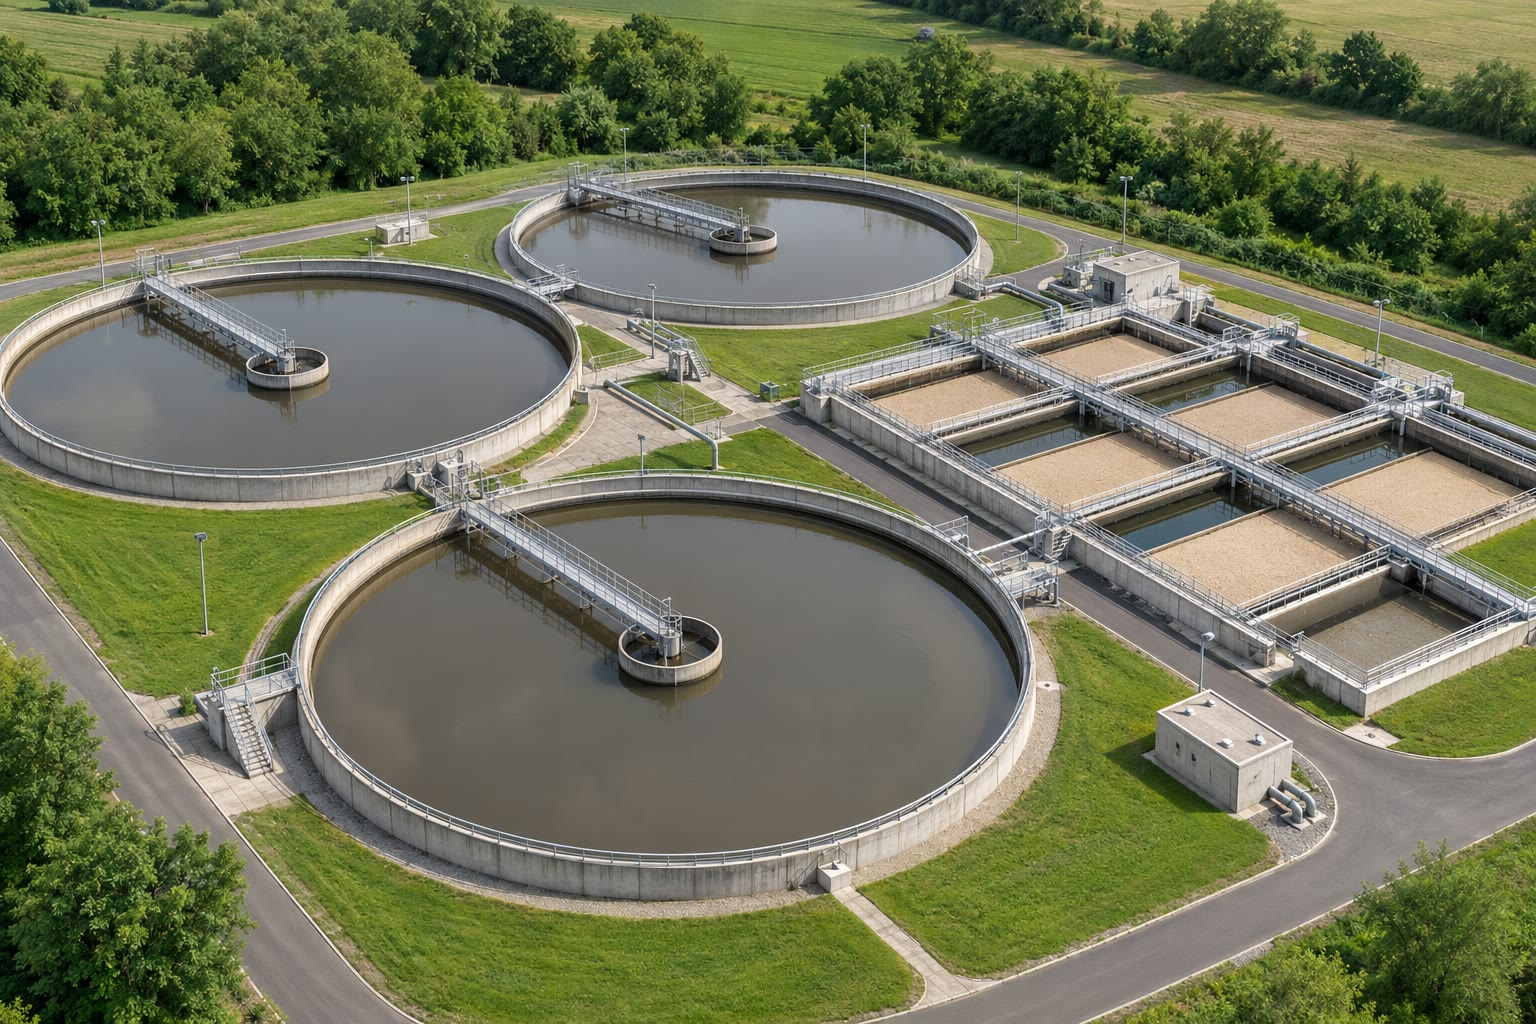
\includegraphics[width=\linewidth,height=4.6cm,keepaspectratio]{images/book1/ai/g3-settling-tanks.jpg}

{\small 净水厂沉降池的照片。}
\end{minipage}\hfill
\begin{minipage}[t]{0.48\linewidth}\centering
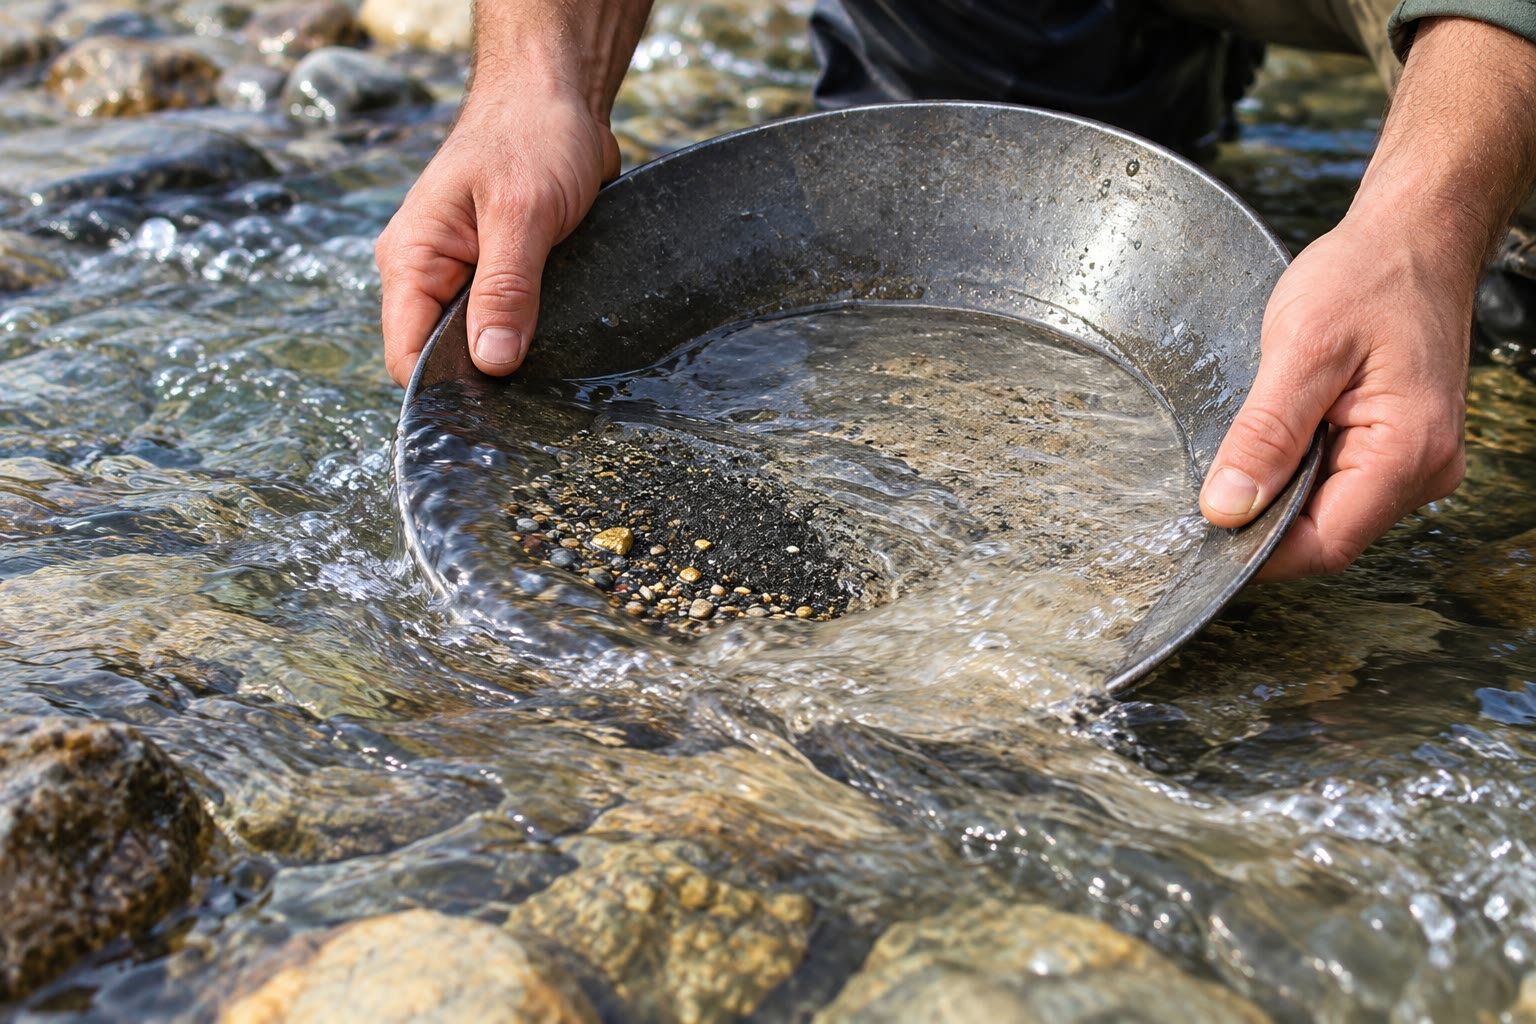
\includegraphics[width=\linewidth,height=4.6cm,keepaspectratio]{images/book1/ai/g3-gold-panning.jpg}

{\small 淘金时，河水会把轻的沙子冲走；
重的颗粒留在盘中。}
\end{minipage}
\end{omfigure}

\begin{remark}[清澈不等于干净]\label{rem:g3:separating-mixtures:clean}
经过过滤的水可能看上去十分清澈，但仍可能含有溶解的物质，
以及小得肉眼看不见的细菌。
因此即使经过过滤，也没有人会直接饮用池塘或溪流中的水。
\end{remark}

\section{练习}

\begin{exercise}[$\star$]\label{exo:g3:separating-mixtures:1}
用哪种方法可以把豌豆和米粒分开？
\end{exercise}

\begin{exercise}[$\star$]\label{exo:g3:separating-mixtures:2}
将一杯泥水放在桌上静置一小时，泥土会发生什么变化？
这种现象叫做什么？
\end{exercise}

\begin{exercise}[$\star$]\label{exo:g3:separating-mixtures:3}
什么是滤液？写出煮咖啡时得到的滤液。
\end{exercise}

\begin{exercise}[$\star$]\label{exo:g3:separating-mixtures:4}
将盐水倒入滤纸中。滤液是咸的吗？
请说明理由。
\end{exercise}

\begin{exercise}[$\star$]\label{exo:g3:separating-mixtures:5}
如何从一杯糖水中把糖取回来？
\end{exercise}

\begin{exercise}[$\star$]\label{exo:g3:separating-mixtures:6}
看一看筛子的图。哪些颗粒留在筛子里？
为什么其他颗粒会漏下去？
\end{exercise}

\begin{exercise}[$\star$]\label{exo:g3:separating-mixtures:7}
将每种混合物与一种方法配对——筛分、过滤或蒸发：
(a) 沙子和卵石；(b) 水中的粉笔粉；(c) 水中的食盐。
\end{exercise}

\begin{exercise}[$\star$]\label{exo:g3:separating-mixtures:8}
看一看净水厂的图。水要经过几个步骤？
哪一步去除了泥沙？
\end{exercise}

\begin{exercise}[$\star$]\label{exo:g3:separating-mixtures:9}
将下列步骤排好顺序，以便从装有沙子、食盐和水的
罐子中取回沙子和食盐：蒸发滤液；过滤；
从滤纸上收集沙子。
\end{exercise}

\begin{exercise}[$\star\star$]\label{exo:g3:separating-mixtures:10}
过滤能否使海水可以饮用？请解释为什么不能。
\end{exercise}

\begin{exercise}[$\star\star$]\label{exo:g3:separating-mixtures:11}
茶壶里装满了茶水，茶叶留在其中。
写出本章中两种能把茶水与茶叶分开的方法。
\end{exercise}
